\documentclass[12pt]{article}

\usepackage{natbib}
\usepackage[left=2cm, right=2cm, top=2cm, bottom=2cm]{geometry}
\usepackage{setspace}
\usepackage{amsmath}
\usepackage{amsthm}
\usepackage{graphicx}
\usepackage{footnote}
\usepackage{threeparttable}
\usepackage{graphics}
\usepackage{dcolumn}
\usepackage{booktabs}
\usepackage{caption}
\usepackage{subcaption}
\usepackage{tikz}
\usepackage[title]{appendix}
\usepackage{pdflscape}

\usepackage[T1]{fontenc}
\usepackage[utf8]{inputenc}
\usepackage{authblk}

\usepackage[labelsep=period]{caption}

\renewcommand*\thetable{\Roman{table}}

\newcommand{\tab}{\hspace*{2em}}

\newtheoremstyle{hypothesis}{0.2in}{0.2in}{\upshape}{}{\itshape}{:}{.5em}{}
\theoremstyle{hypothesis}
\newtheorem{hypothesis}{\it Hypothesis}

\title{The complex structure of commercial peace \\ \Large{Contrasting trade interdependence, asymmetry and multipolarity}}

\author[*]{Erik Gartzke}
\author[**]{Oliver Westerwinter}
\affil[*]{Department of Political Science, University of California, San Diego}
\affil[**]{Department of Political Science, University of St. Gallen}

\renewcommand\Authands{and}

\date{}

\begin{document}

\maketitle

\vspace{2cm}

%\begin{center}
%\textit{Work in progress}
%\end{center}

%\vspace{2cm}

\begin{abstract}

\noindent Researchers continue to debate the impact of trade on interstate conflict. While many view trade as pacifying, others argue that dependencies add to friction and war. We provide a theory that explains how cross-border economic ties alternately enhance or impede international cooperation.  Three main factors account for the heterogeneous effects of trade on conflict:  interdependence, asymmetry and multipolarity.  Interdependence can act as a substitute for, or as a deterrent to, militarized violence.  In the former case, interdependence actually increases more modest non-militarized conflict, while also discouraging militarized disputes.  Asymmetry diminishes the conflict-inhibiting effect of trade ties, as dependency cannot simultaneously be used to coerce and to inform.  Multilateral trade networks alternately moderate or enhance the bilateral effects of interdependence and asymmetry on interstate peace.  Our theory and evidence reveal complex, cross-cutting consequences of economic interdependence on conflict behavior and also demonstrate effects well beyond the dyad, suggesting the need to include extra-dyadic ties in future theoretical and empirical research studying the commercial peace.\\

\noindent Keywords: interstate conflict, trade interdependence, asymmetry, multipolarity, networks\\

\noindent Corresponding author: oliver.westerwinter@unisg.ch\\

\end{abstract}

\thispagestyle{empty}

\newpage

\section*{Introduction}

\noindent\doublespace Research on the relationship between trade and conflict is both durable and dialectical, with optimists \citep{Montesquieu:1989,Cobden:1903,angell:1909,rosecrance:1985} and a more heterogeneous group of pessimists \citep{Thucydides:1985,Lenin:1975,carr:1939,waltz:1999}. Liberal theory emphasizes the pacific effects of commerce on world politics \citep{Oneal:1997,Polachek:1997,Pevehouse:2004}. A more diverse tradition argues that trade dependencies actually exacerbate cross-border tensions \citep{Krasner:1976,Waltz:1979,Grieco:1988,Gasiorowski:1986}. Despite sustained interest and effort, it has proven difficult to resolve this dialectic empirically. While the balance of evidence favors the commercial peace, results are often weak or attenuated \citep{Barbieri:1999,Mansfield:2001,Mansfield:2003a,Schneider:2014}.

Why has evidence for the commercial peace remained relatively weak?  We argue that this ambiguity stems from the fact that trade ties generate not one relationship, but several. Trade may affect states' decisions to fight by shaping the opportunity costs that nations face in going to war \citep{Russett:2001,Polachek:1980,Polachek:2010}. Trade relationships could also serve as a means to signal resolve to adversaries in disputes over issues about which states continue to care \citep{Gartzke:2001,Gartzke:2007,Morrow:1999b}. Some aspects of trade could discourage warfare, while other aspects appear more likely to facilitate, or even encourage, interstate conflict.  Distinguishing among disparate consequences of commerce on conflict is critical for improved theory and for proper assessment of these empirical relationships.

Conflict occurs because states possess incompatible interests, and because adversaries are unwilling or unable to resolve differences non-violently \citep{fearon:1995}. The prospect of trade losses can discourage conflict where the risk posed to commerce from fighting is large relative to the value of the stakes in a dispute.  To deter conflict, trade partners must prefer the status quo to making, or resisting, demands for change.   However, militarized conflicts tend already to be costly; additional incremental burdens due to trade are unlikely to significantly alter states' calculations of risk and return.  If the cost of fighting varies with the intensity of a dispute, then the deterrent effect of commercial ties should do more to alter the intensity of contests than their propensity.

While trade can deter, it can also inform.  Trade ties provide a novel mechanism allowing states to act out their differences through non-militarized conflict.  Indeed, trade can substitute for force; trading relationships need only be valuable to both sides in a dyad. To the degree that interdependence mimics key attributes of militarized contests, it can supplant more deadly or risky disputes.  However, interdependence does not necessarily imply the end of disagreement among states. Tensions may persist and while they are less likely to produce casualties, trading partners may actually {\it increase} incidents of low-intensity non-militarized conflict \citep{Gartzke:2003}.

Asymmetric trade relationships undermine the pacific effects of commerce by decoupling the dual functions of conflict \citep{Hirschman:1945,Keohane:1977}. The less dependent partner in an asymmetric trade relationship can coerce, but this actor does not incur a significant cost for doing so. Coercing cheaply is not informative and so adversaries must find some way to impose costs on a less dependent adversary in order to test resolve. The more dependent state in an asymmetric trade relationship can demonstrate resolve, but it derives little benefit from doing so, given that the less dependent state cannot be coerced through the exercise of the trade mechanism.

These tendencies actually reverse themselves to some degree with increasing extra-dyadic trade ties.  Multilateral asymmetric trade networks---i.e. situations in which states have asymmetric trade ties to more than one state---should be less conflict prone than isolated asymmetric trade relationships. Increasing extra-dyadic trade ties means that both states in an asymmetric network are able to substitute away from a given dyadic dependency.  For the dependent state, a network of dependent relationships tends to undermine the coercive leverage of the less dependent state and thus limits the need to escalate conflict within the dyad to resist coercion. Similarly, for the less dependent partner in an asymmetric trade dyad, increasing the number of asymmetric ties creates more opportunities for coercion, marginally lowering the utility of coercing any particular partner.

The complex, contrasting tendencies of trade networks continue for symmetric (interdependent) dyads. Increasing the number of a state's symmetric trade ties again leads to the opportunity for substitution, but this time the effect is to \textit{decrease the decrease} in conflict associated with bilateral interdependence.  Symmetric trade networks reduce the constraining effect of interdependence on conflict and can also limit the informational value of competition through commercial ties. In short, extra-dyadic trade ties are likely to shape the way that dyadic dependence and interdependence affect interstate conflict, something that scholars have only recently begun to assess systematically \citep{Crescenzi:2005,Martin:2008,Dorussen:2010,Kinne:2012,Kinne:2014b}.

This study begins the process of evaluating these admittedly complex and countervailing tendencies. Complexity is increased by our decision to address trade and conflict from an explicitly networked perspective. Bringing economic networks into the analysis of trade and conflict is essential in unraveling the multiple causal pathways through which commerce operates on war and peace. By doing so, we are better able to explain previous empirical riddles and to provide a larger, more comprehensive theoretical framework for assessing the commercial peace. Our analysis also serves as an illustration of how network theory and measures can be applied to enrich existing theoretical arguments and empirical models in the study of international conflict. In doing so, we add to a growing literature on networks in international relations that has begun to show how the accumulation of ties among nations affect a broad range of international outcomes \citep{Maoz:2011,Dorussen:2008,Ward:2016,Hafner:2008,Hegre:2010,Lupu:2016,Wilson:2016,Chyzh:2016}.

The main conclusion of our analysis is that extra-dyadic trade ties tend to reduce the effects of dyadic trade relationships in tempering or inflaming conflict. Asymmetric dyadic trade dependencies generally increase the likelihood of conflict. Symmetric dyadic trade dependencies (interdependence) tend to reduce the likelihood of militarized conflict.  However, symmetric dyadic dependencies increase non-militarized disputes. Asymmetric extra-dyadic trade relationships of both the more and less dependent state in the dyad mitigate the negative effects of dyadic asymmetric dependence on militarized conflict. In short, our analysis shows that networked trade dependencies lessen the impact of dyadic trade relationships.  Combined with a better understanding of the countervailing tendencies of bilateral trade ties, recognition that extra-dyadic trade ties temper bilateral effects helps to reconcile existing controversies concerning trade and conflict.

The next section details our theory and develops hypotheses on how dyadic and extra-dyadic trade relationships affect tendencies toward war and peace. We then discuss our research design. The third section presents the results of our empirical analysis. A final section concludes.

\section*{Theory: The push and pull of commerce}

In its simplest form, our argument is that complexity may account for ambiguity in the observed effects of commerce on conflict. Trade ties produce several effects, each of which has different consequences for cooperation and conflict.  We characterize these effects as asymmetry, interdependence and multipolarity, discussing each below.  Before doing so, however, we begin by delineating our theory of conflict.  Any attempt to explain how one process, such as trade, affects a second process, such as conflict, must begin with a baseline causal account.  Otherwise, theory is incomplete and claims cannot be evaluated empirically.  Whether trade impacts conflict in one or several ways, it does so by altering the conditions that lead states to fight (or not) in the absence of commercial ties.  To matter for war, trade must change whatever it is that triggers the decision to fight, whether this involves opportunity costs, information, or institutional or other constraints.

\subsection*{Conflict}

States or other actors fight when they have different interests and when they are unable to resolve differences through less costly means.  Most wars, and just about all lesser disputes, end in negotiated compromises, not through a military decision.  This implies that deals typically exist that states come to accept \textit{eventually}.  The causes of war can then be attributed to whatever prevents states from forging the deals that end wars, before fighting begins \citep{Blainey:1973,Morrow:1989,fearon:1995,powell:1999}.  War itself is therefore a process of discovery or transformation, where parties that could not agree on bargains find compromises each prefers to continued fighting.

On its surface, negotiation seems clearly more efficient than war.  However, states may be unable to negotiate effectively for at least three reasons \citep{fearon:1995}.  First, one or more competitors may not know the willingness or ability of other actors to compromise.  Combined with incentives to compete, uncertainty can prevent the forging of mutually acceptable bargains \citep{Morrow:1989,fearon:1995}.  Actors with less bargaining power can increase their leverage by lying about factors affecting various aspects of a contest.   Bluffing can in turn lead opponents to err in making adequate offers when counterparts are in fact capable, cost tolerant or resolved.  Second, goods or issues in dispute may not be divisible, preventing the realization of mutually acceptable compromises. Finally, acceptable bargains may not be self-enforcing \citep{Powell:1996a,Powell:2006}. The most familiar example of so called commitment problems involves power transition, where predictable changes in the future distribution of power lead the declining power to prefer fighting today, rather than being forced into concessions tomorrow \citep{Organski:1958,Organski:1980}.

%\footnote{If states fight because compromises are unavailable, war must make compromises available for fighting to end.}
%\footnote{\citet{fearon:1995} assumes that fighting is costly.  Actors could potentially derive consumption value from fighting.}

Trade can potentially impact the causes of conflict in several ways.  However, the number of ways that interact most plausibly with the theory of warfare outlined above is rather more limited.  For trade to act as a barrier to conflict, for example, the commercial losses anticipated from fighting must be large relative to the overall cost of fighting.  Relatively few bilateral trade relationships are substantial enough to accomplish this, though more will apply to minor versus major disputes.  Trading states also tend to be prosperous and are therefore capable of inflicting (and absorbing) high conflict costs.  This does not rule out opportunity cost (i.e. deterrence) arguments \citep{Polachek:2010}, but it does imply that the effects of trade will depend on the nature of conflict.

\subsection*{Interdependence}

Conflict consists of harming and being harmed.  Actors harm in order to compel or to favorably alter the balance of power.  Destruction weakens an opponent's productive capacity, prosperity or material might, advantaging adversaries.  The prospect of future harm can also induce compromise or acquiesce, obviating the need for actual force.  Bargains that were previously unacceptable become appealing, even as deals that were once preferred become less attractive to the winning side \citep{Wittman:1979}.  By harming and being harmed, states eventually become better informed about the private information that initially led to bargaining failure and war \citep{Powell:2004}.

One way to avoid war is to find mechanisms that proxy for fighting.  Alternatives to violence must prove costly for both sides in a dispute.  The ability to impose harm makes an action attractive to actors interested in influencing or weakening an adversary.  The necessity of absorbing harm makes a given method informative.  The difficulty in finding alternatives to military violence as a way of simultaneously imposing and incurring harm has led to its persistence in political affairs.  Actors fight to win, to advantage themselves over others.  However, it is the willingness to suffer that convinces adversaries to act with discretion. Interdependence allows actors to impose costs on one another, but to do so, actors must also incur harm, and further risk retaliation. Interdependence allows contests that are costly and risky, and therefore informative \citep{Morrow:1999b}.

%\footnote{Again, the other alternative states have is to fight total war, but this is rare precisely because it is so costly.}

Interdependence can serve as a vehicle for defusing violence by shifting conflict behavior to lower, non-militarized levels.  Competing through economics rather than warfare makes the use of force unnecessary if the economic costs incurred and imposed are sufficiently informative. If interdependence informs, then trading states should tend to substitute non-militarized for militarized conflict, doing more to reduce the intensity of disputes than to lower frequency \citep{Gartzke:2003}.

\subsection*{Asymmetry}

Interdependence can deter as well as inform.  However, to do this, the value of trade must be sufficient to change the ordinal preferences of actors over the issues at stake in a dispute.  This may often turn out to be even more difficult than the requirement that trade ties be valuable relative to the costs of militarized conflict.  Given the zero-sum nature of contests, changes in the balance of power, cost or risk that discourage one state from acting aggressively encourage increased aggression from the other side.  Deterrence involves increasing the costs or risks of an attack and maintaining or reducing incentives to exploit newfound advantages with larger demands.  As Theodore Roosevelt put it, deterrence requires that one ``speak softly'' {\it and} ``carry a big stick.''  By itself, a big stick will not yield deterrence because the big stick can be used to compel, rather than just to deter.  To the extent that the ability to harm, or equivalently the ability to take away benefits, is used to coerce concessions, the effect of trade as a deterrent to conflict is reduced.

Peace requires that both sides in a dispute prefer the status quo or a negotiated bargain to the costly lottery of war \citep{fearon:1995}.  Trade can be a reason to prefer peace where both sides view the economic costs of a contest as more onerous than the likely fruits of victory.  This is much less likely where the benefits of trade are asymmetric. If one economy is much more dependent on a given bilateral trade relationship than its partner, then the less dependent state can use the relationship to coerce. However, doing so is not particularly informative because the coercing state is not dependent on its partner.  Similarly, the dependent state can demonstrate resolve through resisting coercion.  But this state has little incentive to do so, given that it cannot reciprocally coerce its partner.  Asymmetric trade relationships thus fail to mimic conflict because they do not link harm imposed with harm incurred. Because one side can coerce, but not inform, there is little reason for the less dependent state to refrain from seeking to redistribute, or for punitive purposes.

%These relationships should not prove informative because the actor that can reveal resolve has no incentive to do so, while the actor that has incentives to use the relationship to coerce reveals little or no private information by doing so.

%The dependent state in an asymmetric trade dyad can inform, but not coerce.  Facing the prospect of economic coercion from its adversary, and unable to resist or respond to this pressure symmetrically, there are more reasons for the dependent state to escalate disputes to the level of militarized threats or violence.\footnote{Anticipating initiators and targets is notoriously complex and ambiguous in its own right.  We simply assert here that dependency for one state in a dyad should be associated with increased militarized conflict in the dyad.}  Dependent states may even be better off deterring economic coercion through escalation designed to signal their resolve and to make coercion appear risky.

%Instead of serving as a substitute or barrier to warfare, asymmetric trade ties augment the coercive power of the less dependent state, opening up a new dimension along which influence may be exercised, without actually diminishing the need to exercise other, deadlier forms of conflict.

\subsection*{Multipolarity}

Increasing the number of bilateral trade ties complicates an already complex picture in several ways.  In particular, multipolarity---i.e. situations in which states have trade ties to more than one state---should tend to attenuate the tendencies just delineated above for interdependence and asymmetry.  Consider again an asymmetric bilateral trade relationship.  Dependent states in a two-state world have limited options; they can knuckle under to coercion from the less dependent partner, or resist---demonstrating resolve by incurring costs and possibly escalating a dispute.

Now imagine that the dependent trade partner possesses additional bilateral relationships.  These additional ties could also be asymmetric.  Even while dependent in each case, the dependent state now has options created by its trade network.  Increasing the number of partners both decreases the leverage available to any given partner (partners can coerce but each bilateral tie is less important) and diversifies risk (the dependent state can shift some trade to another partner).\footnote{Researchers have also measured the sensitivity of states to changes in the supply of particular traded goods \citep{Gasiorowski:1986,Polachek:1999,Crescenzi:2003}.  States with domestic markets that are inelastic in their demand for certain goods are more dependent than states with markets that can readily substitute other goods or suppliers for a given traded good.  This approach complements our own; increasing trade partners should generally increase elasticities to the degree that trade partners act as substitutes for a given good. However, use of elasticities limits available data.  It is also not clear that aggregate bilateral trade statistics are necessarily problematic for our purposes, since our hypotheses involve average effects.  Future research might explore how elasticities further modify the behavior of interdependent trade networks, either enhancing or diminishing the effects we examine here.}

A similar logic applies to the less dependent state in an asymmetric trade relationship. As the number of extra-dyadic relationships in which the less dependent state in the dyad is also the less dependent trade partner increases, the less dependent state has more relationships to choose from in deciding which state to coerce.  This should lead to a decrease in the marginal utility for coercing any given partner because of the availability of a larger number of potential targets.

The effect of extra-dyadic trade dependencies in lessening dependence, coercion and conflict could easily be missed if one were to focus exclusively on bilateral trade ties.  Two pairs of asymmetric trade ties with the same nominal characteristics should behave differently, depending on whether the more dependent state is uniquely dependent on one partner or whether dependence is distributed across multiple bilateral relationships. Asymmetrically dependent dyads where the more dependent state has no or only a few extra-dyadic trade partnerships should experience more conflict, while those where the dependent state has a large number of extra-dyadic trade ties should experience less conflict. Likewise, two otherwise identical asymmetric trade relationships should differ in their conflict behavior depending on whether the less dependent state has other relationships in which it is also the less dependent state. Asymmetric dyads, where the less dependent state has no or only a few extra-dyadic trade partnerships, should be more conflict prone, while less dependent states with many extra-dyadic trade ties should experience less conflict.

Economic ties beyond the dyad should also impact symmetric trade ties, weakening cooperation rather than encouraging it. Imagine again a solitary, but symmetrically dependent, dyad. Increasing trade ties should make it possible for a dyadic counterpart to substitute away from a particular relationship in the event of conflict. In opportunity cost/deterrence terms, marginal reductions in a state's reliance on a given trade relationship will tend to make the state less reluctant to press its demands. Additional trade ties also tend to undermine the signaling value of interdependence, since adversaries have more options beyond the dyad. Even nominally symmetric benefits can turn into a vehicle for coercion when one party is better able to take the relationship to the brink.

\subsection*{Hypotheses}

We next draw testable implications from the framework detailed above.  Figure \ref{fig1:extradyadicties} illustrates key relationships leading to six hypotheses.  First, in isolation, symmetric trade ties should tend to discourage interstate conflict.  Figure 1a therefore indicates a negative sign next to ``no extra-dyadic interdependent tie.''  While this prediction is conventional, controversy continues about how trade encourages peace.  If trade deters conflict by creating opportunity costs, then it is the prospect of losses that is critical \citep{Polachek:2010}.  Big, militarized disputes should be less affected in most cases than contests of more modest scope, since the loss of trade is finite and bigger disputes are more expensive.  Smaller, non-militarized conflicts should be most affected, since trade losses most alter the overall cost of small contests and since the risk of escalation should also deter.

\begin{figure}[!t]
\begin{minipage}[t]{1\textwidth}
	\begin{minipage}[t]{.45\textwidth}
			\begin{center}
				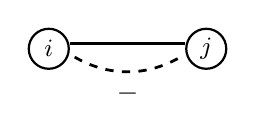
\begin{tikzpicture}
					[dot/.style={circle,minimum height=0.2in,inner sep=0in,draw=black!100,fill=black!00,thick},
					every label/.style= {red}]]
					\node[dot] (i) at (0,0) {\small{$i$}};
					\node[dot] (j) at (2,0) {\small{$j$}};
					\path ([yshift=2pt]j.west) edge[line width=1pt] ([yshift=2pt]i.east);
					\path[dashed] ([yshift=-2pt]i.east) edge[-, bend right, bend angle=45, shorten >=2pt, shorten <=2pt, line width=1pt] node[yshift=-8pt]{$-$} ([yshift=-2pt]j.west);
				\end{tikzpicture}
				\\(a) No extra-dyadic interdependent tie
				\\\vspace{30pt}
				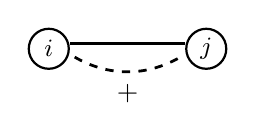
\begin{tikzpicture}
[dot/.style={circle,minimum height=0.2in,inner sep=0in,draw=black!100,fill=black!00,thick},
					every label/.style= {red}]]
					\node[dot] (i) at (0,0) {\small{$i$}};
					\node[dot] (j) at (2,0) {\small{$j$}};
					\path ([yshift=2pt]j.west) edge[line width=1pt] ([yshift=2pt]i.east);
					\path[dashed] ([yshift=-2pt]i.east) edge[-, bend right, bend angle=45, shorten >=2pt, shorten <=2pt, line width=1pt] node[yshift=-8pt]{$+$} ([yshift=-2pt]j.west);
				\end{tikzpicture}
				\\(c) No extra-dyadic asymmetric tie
			\end{center}
	\end{minipage}
	\begin{minipage}[t]{.45\textwidth}
		\begin{center}
				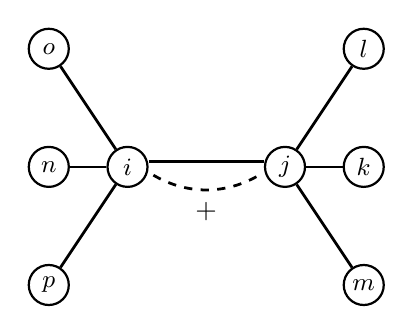
\begin{tikzpicture}
					[dot/.style={circle,minimum height=0.2in,inner sep=0in,draw=black!100,fill=black!00,thick},
					every label/.style= {red}]]
					\node[dot] (i) at (0,0) {\small{$i$}};
					\node[dot] (j) at (2,0) {\small{$j$}};
					\node[dot] (k) at (3,0) {\small{$k$}};
					\node[dot] (l) at (3,1.5) {\small{$l$}};
					\node[dot] (m) at (3,-1.5) {\small{$m$}};
					\node[dot] (n) at (-1,0) {\small{$n$}};
					\node[dot] (o) at (-1,1.5) {\small{$o$}};
					\node[dot] (p) at (-1,-1.5) {\small{$p$}};					
					\path[-] (j) edge [-,line width=1pt] (l);
					\path[-] (j) edge [-,line width=1pt] (k);
					\path[-] (j) edge [-,line width=1pt] (m);
					\path[-] (i) edge [-,line width=1pt] (n);
					\path[-] (i) edge [-,line width=1pt] (o);
					\path[-] (i) edge [-,line width=1pt] (p);
  					\path ([yshift=2pt]j.west) edge[line width=1pt] ([yshift=2pt]i.east);
					\path[dashed] ([yshift=-2pt]i.east) edge[-, bend right, bend angle=45, shorten >=2pt, shorten <=2pt, line width=1pt]node[yshift=-8pt]{$+$} ([yshift=-2pt]j.west);
\end{tikzpicture}
				\\(b) Multiple extra-dyadic interdependent ties $i$ and $j$
				\\\vspace{30pt}
				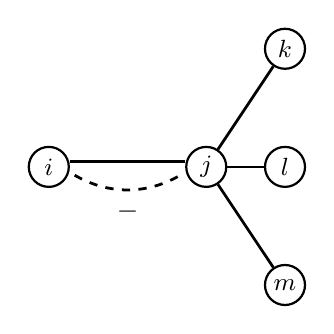
\begin{tikzpicture}
						[dot/.style={circle,minimum height=0.2in,inner sep=0in,draw=black!100,fill=black!00,thick},
					every label/.style= {red}]]
					\node[dot] (i) at (0,0) {\small{$i$}};
					\node[dot] (j) at (2,0) {\small{$j$}};
					\node[dot] (k) at (3,1.5) {\small{$k$}};
					\node[dot] (l) at (3,0) {\small{$l$}};
					\node[dot] (m) at (3,-1.5) {\small{$m$}};
					\path[-] (j) edge [-,line width=1pt] (k);
					\path[-] (j) edge [-,line width=1pt] (l);
					\path[-] (j) edge [-,line width=1pt] (m);
  					\path ([yshift=2pt]j.west) edge[line width=1pt] ([yshift=2pt]i.east);
					\path[dashed] ([yshift=-2pt]i.east) edge[-, bend right, bend angle=45, shorten >=2pt, shorten <=2pt, line width=1pt]node[yshift=-8pt]{$-$} ([yshift=-2pt]j.west);
				\end{tikzpicture}
				\\(d) Multiple extra-dyadic asymmetric ties $j$
		\end{center}
	\end{minipage}
\vspace{15pt}\\
\caption{Extra-dyadic interdependent and asymmetric trade ties and interstate conflict\label{fig1:extradyadicties}}\vspace{10pt}
\caption*{Solid lines indicate bilateral trade relationships. Dashed lines indicate prospective conflict. Subfigures $a$ and $b$ indicate interdependent bilateral trade relationships, while subfigures $c$ and $d$ are asymmetric trade relationships.}
\end{minipage}
\end{figure}

In addition to deterring, trade can also substitute for violence in acting out conflict.   Economic conflict can replace militarized disputes if trade facilitates the dual functions of harming and informing.  Yet, rather than deterring conflict that is most affected by the costly loss of trade, the informational logic implies that symmetric ties actually \textit{increase} minor, non-militarized conflict.  At the same time, because conflict that is informative at lower intensities supplants more intense violence, interdependence should disproportionately reduce militarized conflict \citep{Gartzke:2003}.

\begin{hypothesis}
%\begin{minipage}[t]{5.5 in}
\upshape Interdependent dyads are less likely to experience militarized conflict.
%\end{minipage}
\end{hypothesis}
\begin{hypothesis}
%\begin{minipage}[t]{5.5 in}
\upshape Interdependent dyads are more likely to experience non-militarized conflict.
%\end{minipage}
\end{hypothesis}

Asymmetric trade dependence has been controversial in a different way.  Still, a synthesis can be had simply by estimating contrasting consequences of commerce together, including both the effect of interdependence and asymmetry.  According to our theory, asymmetry undermines the pacific effects of trade by decoupling the dual functions of conflict, informing but not allowing coercion for one side while allowing an adversary to coerce in ways that are not especially informative.

\begin{hypothesis}
\begin{minipage}[t]{5.5 in}
\upshape Asymmetrically dependent dyads are more likely to exhibit militarized conflict.
\end{minipage}
\end{hypothesis}

Extra-dyadic ties should tend to weaken or reverse the effects detailed in the bilateral hypotheses above.  States with multiple dependencies can more effectively counter the coercive effect of any given dependency, limiting usable leverage for less dependent partners and discouraging coercion by less dependent trade partners.  Dependent states therefore have less need to escalate conflicts to counter (less effective) coercion. Similarly, less dependent states with multiple asymmetric trade ties should be less likely to target any particular partner with coercion.  Conflict should decrease in the number of extra-dyadic dependencies for the less dependent state in an asymmetric dyad.

\begin{hypothesis}
\begin{minipage}[t]{5.5 in}
\upshape The tendency for asymmetry to increase militarized conflict should decline in the number of asymmetric partners of the more dependent state in a dyad. \end{minipage}
\end{hypothesis}

\begin{hypothesis}
\begin{minipage}[t]{5.5 in}

\upshape The tendency for asymmetry to increase militarized conflict should decline in the number of asymmetric partners of the less dependent state in a dyad. \end{minipage}
\end{hypothesis}

Finally, symmetric trade ties should be less pacifying when states have numerous trade partners.  States signal resolve to the degree that they endure costs for damaging or suspending trade relationships.  The ties themselves may also deter.  To the degree that states possess a network of trade relationships, ties become a ``substitute for the substitute,'' reducing in particular the informational value of a particular bilateral trade linkage.  The cost of harming a given symmetric bilateral tie is reduced, and the inhibiting or informational effect of a given bilateral relationship declines.  While some informational value is retained as long as existing trade linkages remain valuable, the effect of networks in weakening the pacific effects of trade should be greatest in the case of opportunity costs, where peace is a function of deterrence, rather than by revealing information.

\begin{hypothesis}
\begin{minipage}[t]{5.5 in}
\upshape The tendency for interdependence to reduce militarized conflict should decline in the number of interdependent trade partnerships used by states in a dyad.
\end{minipage}
\end{hypothesis}

\section*{Research design and data}

Testing our hypotheses involves examining the effect of interdependence, asymmetry, and multipolarity of trade on both militarized and non-militarized conflict. Our hypotheses make predictions about the frequency of conflict events. We therefore measure conflict as the number of conflictive events occurring between two states in a given year. We use three dependent variables that count all conflicts, militarized conflicts, and non-militarized conflicts in an undirected dyad-year. We lead the dependent variables by one year to limit reverse causation.

Standard data sources such as the Correlates of War Militarized Interstate Dispute (MID) dataset only code for militarized conflict. The MID dataset and the International Conflict Behavior dataset (ICB) also sample on conflict intensity \citep{Smith:1998,Brecher:1997}. Conflict data thus omit or under-represent the non-militarized conflict needed to evaluate some of our hypotheses. We, therefore, refrain from using the MID and ICB data to test our hypotheses.

Events data seek to code all observations of a given category of behavior within a certain spatial-temporal domain.  They are thus better suited to the objectives of our analysis. We use two different conflict events datasets to code the dependent variables, the Conflict and Peace Data Bank (COPDAB) 1948-1978 and the World Event Interaction Survey (WEIS) 1966-1992. Use of two datasets makes it easier to notice statistical anomalies or artifacts. The COPDAB data scales conflict from 8 (`neutral or non-significant acts for the inter-nation situation') to 15 (`extensive war acts causing deaths, dislocation or high strategic costs') \citep{Azar:1993}. The WEIS data are non-parametric, with no explicit measure of conflict intensity \citep{McClelland:1983}. However, \citet{Goldstein:1992} provides a scheme for scaling WEIS events along a single ordinal conflict dimension that ranges from $0$ (`explain or state policy; state future position') to $-10$ (`military attack; clash; assault').\footnote{We recode $0$ values on the Goldstein scale as $-0.01$ to empirically distinguish `explain or state policy; state future policy' events from dyads that do not experience any conflict. For interpretational reasons, we also translate the negative numbers of the Goldstein scale into positive numbers by taking their absolute values.} An alternative coding scheme to scale WEIS events data along an ordinal conflict dimension was proposed by \citet{Vincent:1979}. The Vincent scale ranges from $2.2$ (`deny') to $4.7$ (`force'). Using WEIS data scaled based on the Vincent scheme yields results that are similar to those presented in this article.\footnote{Results are available from the authors.} In addition to including all conflict events, we include observations for all dyad years in the temporal-spatial domain for which there are no conflict events, so as to avoid selecting on the dependent variable.

To code the conflict dependent variable from COPDAB, we count COPDAB events at scale 9 ``mild verbal expressions displaying discord in interaction'' or higher and sum these events for each undirected dyad-year. For WEIS, we create a dummy variable that is coded $1$ for events that are coded as larger than $0$ on the Goldstein scale and again sum all events for each undirected dyad-year.

The `right' division of conflict behavior between militarized and non-militarized can be debated. Results do not appear sensitive to minor coding changes. In the COPDAB sample, we code scale 11 `diplomatic-economic hostile actions' and scale 12 `political-military hostile actions' as non-militarized conflict and compute the sum of all non-militarized conflict events for each undirected dyad year. We code militarized conflict from COPDAB as scale 13 `small-scale military acts,' 14 `limited war acts,' and 15 `extensive war acts' and again sum the event count in each undirected dyad year. In the WEIS data, we code militarized conflict as beginning in the Goldstein scale at 8.7 `non-military destruction/injury'. Non-militarized conflict are up to 5.8 `threat with specific negative non-military sanction' on the Goldstein scale.\footnote{We omit events that are difficult to categorize, including 6.9 `ultimatum; threat with negative sanction and time limit,' 7 `break diplomatic relations,' 7.6 `armed force mobilization, exercise, display; military buildup,' and 8.3 `non-injury destructive action'.} We again sum the count in undirected dyad-years.

We use data from \citet{Gleditsch:2002} to measure cross-border trade and gross domestic product (GDP).  Dependence is measured as the sum of bilateral imports plus exports from a particular trade partner for a country, divided by its GDP: $Dependence_{i} = \frac{Import_{ij}+Export_{ij}}{GDP_{i}}$ \citep{Oneal:1996}. We take the natural logarithm of this variable to create our base monadic dependence measure. Based on this measure, we construct variables for the lower of two dependence values in the dyad and for the absolute difference between the two monadic dependence values. The lower monadic trade dependence captures economic interdependence, while the absolute difference in trade-weighted GDP measures dyadic asymmetry in dependence.

We construct three additional variables to measure the effects of extra-dyadic trade dependence. First, we capture the potential ability of the more dependent state in a dyad to avoid coercion by substituting away from dependence on a given partner.  {\it{Extra-dyadic asymmetric dependence}}$_{j}$ sums the count of trade relationships in a given year in which the more dependent state in a dyad, $j$, is also more dependent vis-{\`a}-vis other states $k$, among all its trade partners $K$ in year $t$, with the exception of state $i$.\footnote{Since our argument about the effects of extra-dyadic dependencies on dyadic dependencies and interdependencies refers to an absolute and not a relative opportunity that scales with the number of states in the international system, we do not standardize our extra-dyadic dependency measures by the size of the international system in a given year.} Let $more~dependent_{jkt}$ be an indicator variable that is coded 1 if $dependence_{jt} > dependence_{kt}$, and 0 otherwise. We can then write:

\begin{equation}
\text{\it{extra-dyadic asymmetric dependence}}_{j} = \sum_{k \neq i}^{K} more~dependent_{jkt}.
\end{equation}

Second, we measure asymmetry in the extra-dyadic dependencies of the less dependent state, $i$, in the dyad by computing the sum of trade ties of state $i$ with states $k$ in a given year $t$ in which $i$ is the less dependent partner. $K$ refers to all states with which $i$ trades in year $t$ except $j$. We create an indicator, $less~dependent_{ikt}$ that is coded 1 if $dependence_{it} < dependence_{kt}$, and 0 otherwise, and define:

\begin{equation}
\text{\it{extra-dyadic asymmetric dependence}}_{i} =  \sum_{k \neq j}^{K} less~dependent_{ikt}.
\end{equation}

The third variable, extra-dyadic interdependence, measures the number of interdependent ties that the states in a dyad have with other states in the system in a given year. To compute this statistic, we first create an indicator that marks relationships between states $i$ and $j$ and third parties $k$ in which the dependency of the less dependent state in that dyad is at least one standard deviation above the sample mean of the lower monadic dependency variable with $\bar{x}_{dependence_{low}}$ denoting the sample mean and $s_{dependence_{low}}$ referring to the sample standard deviation of the lower monadic dependence variable. For state $i$, this interdependence indicator is coded 1 if $dependence_{low_{ikt}} \geq \left(\bar{x}_{dependence_{low}}+s_{dependence_{low}}\right)$ an 0 otherwise. Analogously, for $j$ it is coded 1 if $dependence_{low_{jkt}} \geq \left(\bar{x}_{dependence_{low}}+s_{dependence_{low}}\right)$ and 0 otherwise. Substantively, this means that we are identifying large trade partnerships, where both states depend on the economic exchange with each other. We then sum these large interdependent trade relationships for states $i$ and $j$ in a given year. We sum the count of both state's large extra-dyadic interdependent ties to measure the extent of networked interdependence for each dyad-year. Equation \ref{eq:equation3} summarizes this statistic formally:

\begin{multline}
\label{eq:equation3}
\text{\it{extra-dyadic interdependence}}_{ij} = \sum_{k \neq j}^{K} interedependence_{ikt} +  \sum_{k \neq i}^{K} interdependence_{jkt}.
\end{multline}

\noindent We interact these measures of extra-dyadic asymmetric dependence and interdependence with our dyadic variables for asymmetric dependence and interdependence to test hypotheses 4-6.

We add a number of econometric controls that have been used in previous research. First, we control for regime type. The Polity IV data provides two eleven-point indexes of regime type based on formal constraints on the executive (AUTOC) and institutional support for democracy (DEMOC) \citep{Jaggers:1995}. We generate monadic regime scores by taking the difference between DEMOC and AUTOC scores, adding ten, and dividing by two $\left(\frac{\left(Democ_{i}-Autoc_{i}\right)+10}{2}\right)$. The resulting measure ranges from $0$ to $10$. We then create two dyadic variables that measure the difference and the lower of the two monadic regime types to capture the effect democracy and regime difference on conflict \citep{Gartzke:2013}.\footnote{In the online appendix, we present robustness checks using the lower and higher monadic regime scores \citep{Choi:2015}. The results are in line with the findings of our main analysis.}

Whether states experience conflict is partly a function of interest compatibility. Measures approximating preference similarity have proven useful in other studies \citep{Mesquita:1981,Gartzke:1998}. Interest similarity has been measured as the correlation between states' alliance portfolios or the similarity of United Nations General Assembly roll-call votes among others. The first approach offers a longer time series, while the latter offers more variance, particularly after World War II. Given the coverage and structure of the COPDAB and WEIS datasets, we adopt the latter approach. We use affinity scores that are based on the ``S'' coding \citep{Signorino:2001} and measure the similarity of states' revealed preferences based on United Nations General Assembly roll-call data \citep{Gartzke:1998}.\footnote{In the online appendix, we provide robustness checks that use alternative measures of preference similarity. The results are in line with the findings of our main analysis.}

Geography is a strong predictor of interstate conflict \citep{Maoz:1993}. We use a measure of two states' direct contiguity and a measure of the distance between the capitals of two states in 1,000 kms to capture the effect of geography on states' likelihood to engage in militarized and non-militarized conflict.

Previous studies include a measure for alliance ties within a dyad \citep{Oneal:1997}. We use the Correlates of War alliance dataset to measure alliance relationships in two ways \citep{Gibler:2009}. First, we code a dummy variable equal to $1$ for any alliance relationship (defense pact, entente, non-agression pact, neutrality), and $0$ otherwise. Second, a similar variable is coded $1$ if states $i$ and $j$ have a formal defense pact or entente and $0$ otherwise. The models in our main analysis use the variable that captures all alliances. Results do not depend on the measure of alliances used.

We also examine the effect of military capabilities on conflict occurrence. This impact is measured using the Correlates of War Composite Indicators of National Capabilities (CINC) \citep{Singer:1987}. We use the CINC of the more powerful state divided by the sum of CINC's in the dyad $\left(\frac{CINC_{high}}{CINC_{i}+CINC_{j}}\right)$. This measure ranges from $0.5$ in situations of perfectly balanced military capabilities to $1$ in situations of perfect imbalance. To control for the effect of economic capacity and the size of a country's economy, we use the lower of the logged monadic GDPs in a dyad.\footnote{In the online appendix, we show that using the lower of the logged monadic population sizes as a proxy for country size does not affect the findings of our main analysis.} Economic development is related to interdependence and might affect a state's willingness to engage in a conflict. To address any concerns about this relationship, we include a dyadic measure that captures the lower of the logged per-capita GDP in the dyad \citep{Oneal:1996,Hegre:2000}.

Finally, we control for temporal dependence using ``peace years'' counts and splines, interpolated from a dummy matrix coding the lag between conflict dyad years in the dependent variable \citep{Beck1998}. The models discussed in the article use ``peace years'' counts and splines based on all conflict behavior. Tables A-2 and A-3 provide summary statistics for the variables used in our main analyses based on the COPDAB data as well as the WEIS data coded using the Goldstein conflict scale.

\subsection*{Model}

Since our dependent variables are event counts, we use count regression methods to estimate our models \citep{Long:1997,Cameron:2013}. Since all three of our dependent variables are characterized by a large number of ``no event'' observations and overdispersion (their variances are many times larger than their means),\footnote{See the online appendix for a more detailed description of our dependent variables.} we use a zero-inflated negative binomial model \citep{Long:1997}. The model assumes that zero outcomes in the data are generated by two distinct processes. One process produces only zeros. A second process produces both zero and non-zero outcomes \citep[242-243]{Long:1997}. The zero-inflated negative binomial model has two parts to capture these two distinct data generating processes, a point mass at zero and a count distribution, which is the negative binomial distribution. Zeros come from either the point mass or the count component \citep[243]{Long:1997}. Let $y_{i}$ be the count of conflict events in dyad $i$ for a given year. For observation $i$ the zero process is chosen with probability $\rho_{i}$ and the count process is chosen with probability $1-\rho_{i}$. Suppose that $h(y_{i})$ is the probability mass function for the counts of conflict events, and $\mathbf{X}_{i}$ is a vector of covariates that affect the frequency with which dyad $i$ experiences conflict if it is generated through the count process. We can write:

\[
 y_{i} = \left\{
  \begin{array}{l c r}
   0 & \text{with probability} & \rho_{i} \\
   h\left(y_{i}|\beta\mathbf{X}_{i}\right)      & \text{with probability} & 1 - \rho_{i}.
  \end{array}
\right.
\]

Using a logistic link function, we model $\rho_{i}$ as a function of covariates that determine selection into zero-only dyads \citep{Long:1997}. Let $\mathbf{Z}_{i}$ be a vector that contains our zero-inflated covariates and $\gamma$ be a vector of zero-inflated coefficients.  We then write $\rho_{i} = F\left(\mathbf{Z}_{i}\gamma\right)$, where $F$ is the logistic cumulative distribution function. Our zero-inflated negative binomial regression is given by the following equation:

\[
Pr(Y_{i}=y_{i}|\mathbf{X}_{i},\mathbf{Z}_{i})= \left\{
	\begin{array}{l c c c r}
		F\left(\gamma \mathbf{Z}_{i}\right) &+ & \left(1-F\left(\gamma 						\mathbf{Z}_{i}\right)\right) h\left(0|\beta\mathbf{X}_{i}\right) & \text{if}& y_{i} =0 \\
		& & \left(1-F\left(\gamma \mathbf{Z}_{i}\right)\right)h\left(y_{i}|\beta\mathbf{X}_{i}\right) & 		\text{if}&  y_{i} > 0,
	\end{array}
\right.
\]

\noindent where $h(y_{i})$ again refers to the probability mass function. We model $\rho_{i}$ as a function of geographic distance and the lower of the logged monadic GDPs in a dyad. We expect that geographically distant states are more likely to experience zero conflict events with certainty than states that are located close to each other. Furthermore, we expect countries with higher levels of economic capacitiy to be less likely to experience zero conflict with certainty.\footnote{In the online appendix, we present results of models with alternative specifications of the zero-inflation component of our estimation. We find that including additional variables in the zero-inflation part of our model does not affect our findings.}

An alternative approach to modeling conflict data is offered by longitudinal network models, such as temporal exponential random graph models (TERGMs) or stochastic actor-oriented models (SAOMs) \citep{Hanneke:2010, Cranmer:2011,Snijders:1996}. These models allow to examine interdependencies among states as a network of states and then estimate the determinants of network structures statistically. Scholars have used these models to study international conflict typically with MID data as basis for identifying network ties \citep{Cranmer:2011,Warren:2016}. However, both TERGMs and SAOMs are currently only available for dichotomous outcome variables. This poses a challenge for modeling count data. Since our argument focuses on the frequency of conflict events between states, it is difficult to use TERGMs or SAOMs to examine our data. We would have to dichotomize our event counts and then use this as basis of a statistical network analysis. This would, however, change the dependent variable and any results that such a model would yield would be challenging to compare to our findings. Given the specific theoretical focus of our analysis, the use of count models is therefore preferable over network models.\footnote{By estimating our models using robust standard errors, we correct for some of the interdependencies that network models would allow us to model more explicitly. In addition, we estimate TERGMs based on a dichotomization of our dependent variables and present the results in the online appendix. The results of these models are in line with the findings of our main analysis.}

\section*{Results}

We start our empirical analysis by investigating our hypotheses on the effect of dyadic interdependence and asymmetric dependence on the frequency of interstate conflict. Table \ref{tab1:copdabdyadicmodels} reports the results of this analysis in three parts.\footnote{We acknowledge that models that include many independent variables have been critized \citep{Achen:2005}. \citet{Achen:2005} in particular argued that econometric models that are specified without the support of a formal model should not contain more than three independent variables. In the online appendix, we present more parsimonious model specifications. The results are in line with the findings of our main analysis.} The upper portion reports results for those observations produced by the count process. The middle portion presents results from modeling the latent process for whether the data generating process is certain to produce zeros. The bottom portion contains model summary statistics. We begin by discussing the results of the inflation models, and then turn to count outcomes and overall model statistics.\footnote{The results that we present in this section have been estimated using listwise deletion to address missing data. In the online appendix, we present results based on imputed missing data. Changing our approach to deal with missing data does not affect the results of our main analysis.}

\begin{table}[htbp]\centering\scriptsize
\def\sym#1{\ifmmode^{#1}\else\(^{#1}\)\fi}
\caption{Zero-inflated negative binomial regression estimates, dyadic interdependence and asymmetric dependence (COPDAB, 1948-1978)\label{tab1:copdabdyadicmodels}}
\begin{tabular}{l*{3}{D{.}{.}{-1}}}
\toprule
   &\multicolumn{1}{c}{(1)}&\multicolumn{1}{c}{(2)}&\multicolumn{1}{c}{(3)}\\
   &\multicolumn{1}{c}{All conflict}&\multicolumn{1}{c}{Mil. conflict}&\multicolumn{1}{c}{Non-mil. conflict}\\
\midrule
Dependence low&      -1.731         &      -1.463         &       2.923\sym{*}  \\
   &     (1.282)         &     (8.642)         &     (1.345)         \\
\addlinespace
Dependence difference&       0.839\sym{***}&       0.281\sym{*}  &                     \\
   &    (0.032)         &     (0.118)         &                     \\
\addlinespace
Regime type low&      0.026\sym{***}&      0.056\sym{*}  &      0.036\sym{***}\\
   &   (0.007)         &    (0.026)         &   (0.009)         \\
\addlinespace
Difference regime type&      0.053\sym{***}&       0.106\sym{***}&      0.051\sym{***}\\
   &   (0.006)         &    (0.024)         &   (0.008)         \\
\addlinespace
Log GDP/capita low&      0.044\sym{+}  &      -0.321\sym{**} &       0.336\sym{***}\\
   &    (0.025)         &    (0.098)         &    (0.031)         \\
\addlinespace
Log GDP low&       0.233\sym{***}&      -0.139\sym{+}  &      0.059\sym{*}  \\
   &    (0.017)         &    (0.082)         &    (0.03)         \\
\addlinespace
Affinity (UNGA)&      -1.452\sym{***}&      -1.514\sym{***}&      -1.478\sym{***}\\
   &    (0.052)         &     (0.210)         &    (0.068)         \\
\addlinespace
Capability ratio&       1.126\sym{***}&       1.044\sym{*}  &       1.170\sym{***}\\
   &     (0.125)         &     (0.467)         &     (0.178)         \\
\addlinespace
Alliances (all types)&       1.072\sym{***}&       0.240         &       0.770\sym{***}\\
   &    (0.045)         &     (0.174)         &    (0.061)         \\
\addlinespace
Distance&      -0.103\sym{***}&     -0.044         &     -0.042\sym{**} \\
   &   (0.006)         &    (0.059)         &    (0.014)         \\
\addlinespace
Contiguity&       1.441\sym{***}&       3.299\sym{***}&       1.421\sym{***}\\
   &    (0.064)         &     (0.181)         &    (0.074)         \\
\addlinespace
Constant&      -4.905\sym{***}&       1.304         &      -5.384\sym{***}\\
   &     (0.361)         &     (1.684)         &     (0.649)         \\
\midrule
Distance&       0.187\sym{***}&       0.231\sym{***}&       0.270\sym{***}\\
   &    (0.016)         &    (0.035)         &    (0.016)         \\
\addlinespace
Log GDP low&      -1.734\sym{***}&      -0.650         &      -1.062\sym{***}\\
   &     (0.204)         &     (0.446)         &     (0.122)         \\
\addlinespace
Contant&       25.59\sym{***}&       9.933         &       15.63\sym{***}\\
   &     (3.107)         &     (6.745)         &     (1.817)         \\
\midrule
Log $\alpha$&       1.900\sym{***}&       3.222\sym{***}&       2.049\sym{***}\\
   &    (0.025)         &     (0.321)         &    (0.063)         \\
Vuong $(z)$&        8.81             &           2.11          &           6.32          \\
Likelihood ratio $\chi^{2}$&     21,434.2\sym{***}         &      2,794.0\sym{***}         &      8,188.6\sym{***}         \\
Log likelihood &    -51,403.686      &         -4,492.353      &       -20,096.432        \\
McFadden's pseudo R$^{2}$&         0.172            &     0.234      &           0.168        \\
Observations&      145,903         &      145,903         &      145,903         \\
\bottomrule
\multicolumn{4}{l}{\scriptsize Robust standard errors in parentheses. Coefficients of ``peace years''}\\
\multicolumn{4}{l}{\scriptsize and splines not reported. All significance tests two-tailed.}\\
\multicolumn{4}{l}{\scriptsize \sym{+} \(p<0.10\), \sym{*} \(p<0.05\), \sym{**} \(p<0.01\), \sym{***} \(p<0.001\).}\\
\end{tabular}
\end{table}


Beginning with the middle section of table \ref{tab1:copdabdyadicmodels}, two states that are far away from each other are more likely to be in the certain zero conflict category. This effect is statistically significant across all three models. By contrast, an increase in the lower of the monadic logged GDPs makes states less likely to be in the zero-only outcome. In other words, dyads that involve states with high levels of economic capacity are likely to experience some conflict. This effect is statistically significant in models 1 and 3 in table \ref{tab1:copdabdyadicmodels}.

Moving to the upper portion of table \ref{tab1:copdabdyadicmodels}, we find that the probability of experiencing general conflict as well as militarized conflict increases as dyadic asymmetry (dependence difference) increases.\footnote{Including or excluding the outlier Korean War observations has no affect on the results in tables \ref{tab1:copdabdyadicmodels} and \ref{tab2:extradyadicdependenciescopdab}.} With respect to all conflict behavior, increasing the absolute difference of two states' logged trade dependence by one standard deviation is estimated to increase the expected number of general conflict events by a factor of $1.5$. Similarly, a one-standard deviation increase in the difference of logged monadic dependencies is associated with an increase in the number of estimated militarized conflict events by a factor of $1.1$. By contrast, we fail to find statistically significant support for our hypothesis that dyadic interdependence is negatively related to conflict in general and militarized conflict.

The coefficients of non-linear models are hard to interpret directly. We therefore compute the predicted number of militarized conflict events as the asymmetric dependence of two states increase. As the left-hand part of figure \ref{fig2:predictednumberevents} shows, holding other variables constant at their means, as the difference in logged monadic dependencies increases, we observe an increase in the number of predicted militarized conflict events between states. While pairs of states with low levels of asymmetric dependence are predicted to experience close to zero militarized conflicts, those with higher levels of asymmetric dependence are predicted to be engaged in more militarized conflict events. These findings lend credence to hypothesis 3.

\begin{figure}
\centering
\begin{minipage}{.5\textwidth}
  \centering
  \includegraphics[width=1\linewidth]{Predicted_Number_Militarized_Conflict_Events_Asymmetric_Dependence_10022016.pdf}
\end{minipage}%
\begin{minipage}{.5\textwidth}
  \centering
  \includegraphics[width=1\linewidth]{Predicted_Number_Non-Militarized_Conflict_Events_Interdependence_10022016.pdf}
\end{minipage}
\caption{Predicted number of militarized and non-militarized conflict events (COPDAB, 1948-1978)}
 \label{fig2:predictednumberevents}
\caption*{Calculations of predicted number of militarized conflict events are based on model 1 in table \ref{tab1:copdabdyadicmodels}. Calculations of predicted number of non-militarized conflict events are based on model 3 in table \ref{tab1:copdabdyadicmodels}. All other variables held constant at their means. 95\% confidence intervals.}
\end{figure}

Model 3 tests hypothesis 2 about the positive effect of dyadic interdependence on non-militarized conflict. This model includes the lower of the two logged monadic dependence values as independent variable to capture dyadic interdependence, but not our measure for asymmetric dependence. We do not include the asymmetric dependence measure because our theoretical argument does not make predictions about the affect of asymmetric dependence on non-militarized conflict. As our results show, a dyad is \textit{more} (not less) likely to experience non-militarized conflict as the threshold trade dependence in a dyad increases. A one-standard deviation increase in the lower of the logged monadic dependencies is a associated with a $1.02$ factor change in the expected number of non-militarized conflicts. States that are more interdependent are estimated to experience more non-militarized conflict events. This finding is supported when we examine the predicted number of non-militarized conflict events as the lower of the logged monadic dependencies increases (see right-hand side of figure \ref{fig2:predictednumberevents}). This result supports hypothesis 2.

The bottom portion of table \ref{tab1:copdabdyadicmodels} provides statistics for assessing model fit. The natural log of $\alpha$ is the dispersion parameter. If dispersion is zero (the variance and mean of the dependent variable are identical), then a Poisson model would be the most appropriate estimator for these data. Since the log of $\alpha$ is statistically different from 1 ($\alpha = 0$), there is significant evidence for overdipsersion.  Use of negative binomial regression is indicated.  We also conduct a Vuong test for each of the models in table \ref{tab1:copdabdyadicmodels}. This test compares the zero-inflated negative binomial model to a standard negative binomial model \citep{Vuong:1989}. The $z$-value of this test is significant for all regressions, confirming that the zero-inflated negative binomial is a better fit for these data.

\begin{table}[htbp]\centering\scriptsize
\def\sym#1{\ifmmode^{#1}\else\(^{#1}\)\fi}
\caption{Zero-inflated negative binomial regression estimates, extra-dyadic interdependence and asymmetric dependence (COPDAB, 1948-1978) \label{tab2:extradyadicdependenciescopdab}}
\begin{tabular}{l*{3}{D{.}{.}{-1}}}
\toprule
   &\multicolumn{1}{c}{(4)}&\multicolumn{1}{c}{(5)}&\multicolumn{1}{c}{(6)}\\
   &\multicolumn{1}{c}{Mil. conflict}&\multicolumn{1}{c}{Mil. conflict}&\multicolumn{1}{c}{Mil. conflict}\\
\midrule
Dependence low&      -0.758         &      -0.996         &      -2.460         \\
   &     (8.037)         &     (8.337)         &     (6.353)         \\
\addlinespace
Dependence difference&       0.625\sym{**} &       0.759\sym{**} &       0.288\sym{*}  \\
   &     (0.227)         &     (0.262)         &     (0.118)         \\
\addlinespace
Extra-dyadic dependencies&      0.015\sym{***}&                     &                     \\
more dependent state   &   (0.004)         &                     &                     \\
\addlinespace
Dependence difference X extra-dyadic&    -0.009\sym{*}  &                     &                     \\
dependencies more dependent state   &   (0.004)         &                     &                     \\
\addlinespace
Extra-dyadic dependencies&                     &      0.012\sym{***}&                     \\
less dependent state   &                     &   (0.002)         &                     \\
\addlinespace
Dependence difference X extra-dyadic&                     &    -0.007\sym{**} &                     \\
dependencies less dependent state   &                     &   (0.003)         &                     \\
\addlinespace
Sum large extra-dyadic trade&                     &                     &     -0.016         \\
 relationships  &                     &                     &    (0.022)         \\
\addlinespace
Dependence low X sum large&                     &                     &       0.175         \\
 extra-dyadic trade relationships  &                     &                     &     (0.418)         \\
\addlinespace
Regime type low&      0.052\sym{*}  &      0.049\sym{+}  &      0.052\sym{*}  \\
   &    (0.026)         &    (0.026)         &    (0.026)         \\
\addlinespace
Regime type difference&      0.098\sym{***}&      0.097\sym{***}&       0.104\sym{***}\\
   &    (0.024)         &    (0.024)         &    (0.023)         \\
\addlinespace
Log GDP/capita low&      -0.372\sym{***}&      -0.337\sym{***}&      -0.306\sym{**} \\
   &    (0.094)         &    (0.098)         &     (0.101)         \\
\addlinespace
Log GDP low&      -0.168         &     -0.036         &      -0.134         \\
   &     (0.124)         &    (0.064)         &    (0.083)         \\
\addlinespace
Affinity (UNGA)&      -1.692\sym{***}&      -1.433\sym{***}&      -1.498\sym{***}\\
   &     (0.202)         &     (0.211)         &     (0.210)         \\
\addlinespace
Capability ratio&       1.168\sym{*}  &       0.813\sym{+}  &       1.042\sym{*}  \\
   &     (0.457)         &     (0.466)         &     (0.468)         \\
\addlinespace
Alliance (all types)&       0.443\sym{*}  &       0.183         &       0.227         \\
   &     (0.177)         &     (0.171)         &     (0.173)         \\
\addlinespace
Distance&     -0.011         &      -0.133\sym{***}&     -0.041         \\
   &    (0.04)         &    (0.022)         &    (0.055)         \\
\addlinespace
Contiguity&       3.188\sym{***}&       3.325\sym{***}&       3.300\sym{***}\\
   &     (0.175)         &     (0.179)         &     (0.181)         \\
\addlinespace
Constant&       1.654         &      -0.767         &       1.135         \\
   &     (2.356)         &     (1.358)         &     (1.721)         \\
\midrule
Distance&       0.234\sym{***}&       0.281\sym{***}&       0.231\sym{***}\\
   &    (0.041)         &    (0.053)         &    (0.035)         \\
\addlinespace
Log GDP low&      -0.403         &      -3.030\sym{***}&      -0.651         \\
   &     (0.297)         &     (0.562)         &     (0.400)         \\
\addlinespace
Constant&       6.253         &       46.45\sym{***}&       9.962         \\
   &     (4.625)         &     (8.641)         &     (6.059)         \\
\midrule
Log $\alpha$&       2.947\sym{***}&       3.530\sym{***}&       3.220\sym{***}\\
   &     (0.283)         &    (0.092)         &     (0.292)         \\
Vuong $(z)$&          2.18            &         3.92              &           2.11          \\
Likelihood ratio $\chi^{2}$&      2,823.2\sym{***}         &      2,839.9\sym{***}         &      2,794.8\sym{***}         \\
Log likelihood&         -4,477.764             &             -4,469.416         &           -4,491.967          \\
McFadden's pseudo R$^{2}$&        0.236             &           0.237           &         0.234             \\
Observations&      145,903         &      145,903         &      145,903         \\
\bottomrule
\multicolumn{4}{l}{\scriptsize Robust standard errors in parentheses. Coefficients of ``peace years'' and splines not reported.}\\
\multicolumn{4}{l}{\scriptsize All significance tests two-tailed. \sym{+} \(p<0.10\), \sym{*} \(p<0.05\), \sym{**} \(p<0.01\), \sym{***} \(p<0.001\).}\\
\end{tabular}
\end{table}


We now turn to tests of hypotheses 4 and 5 on the effect of the interaction of dyadic and extra-dyadic asymmetric dependence on militarized conflict. We again start at the middle section of table \ref{tab2:extradyadicdependenciescopdab}. The general results for selection into no militarized conflict with certainty repeat the findings from table \ref{tab1:copdabdyadicmodels}. Distant dyads are more likely to be certain to experience no militarized conflict, while dyads that include states with high economic capacity are less likely to not engage in militarized conflict with certainty. Moreover, looking at the bottom part of table \ref{tab2:extradyadicdependenciescopdab}, we see that the zero-inflated negative binomial regressions are again a better fit than alternative estimators.

Moving to the results for the count portion of the models, we can see from column 1 of table \ref{tab2:extradyadicdependenciescopdab} that the positive effect of asymmetric dependence on militarized conflict decreases with the number of extra-dyadic asymmetric trade partnerships of the more dependent state in the dyad. Model 5 finds a similar effect for the interaction between dyadic asymmetric dependence and the number of extra-dyadic asymmetric dependencies of the less dependent state in the dyad. As the number of extra-dyadic dependencies of the less dependent state in the dyad increases, the militarized conflict producing effect of dyadic dependence decreases. The destabilizing effect of dyadic asymmetric trade dependency is mitigated by a network of extra-dyadic trade dependencies.

We plot the average marginal effects of dyadic asymmetric dependence on militarized conflict in a dyad for different levels of extra-dyadic dependence of the more dependent state in a dyad in figure \ref{fig3:asymmetricdependenceinteraction}. As the figure reveals, the tendency for dyadic asymmetric dependence to increase the expected number of militarized conflicts decreases in the number of extra-dyadic  dependencies of the more dependent state in a dyad. The effect of dyadic asymmetry even becomes statistically insignificant for dyads where the more dependent state has many extra-dyadic asymmetric trade ties. Thus, extra-dyadic network dependencies of the more dependent state in a dyad decrease the conflict enhancing effect of asymmetric dyadic trade dependence. We find a similar effect of the extra-dyadic dependence of the less dependent state in the dyad on the conflict-enhancing effect of dyadic asymmetric dependence.

\begin{figure}
\centering
\begin{minipage}{.5\textwidth}
  \centering
  \includegraphics[width=1\linewidth]{Interaction_Asymmetric_Dependence_More_Dependent_State_Mil_Conflict_10022016.pdf}
\end{minipage}%
\begin{minipage}{.5\textwidth}
  \centering
  \includegraphics[width=1\linewidth]{Interaction_Asymmetric_Dependence_Less_Dependent_State_Mil_Conflict_10022016.pdf}
\end{minipage}
\caption{Interaction dyadic dependence and extra-dyadic dependence more and less dependent state (COPDAB, 1948-1978)}
 \label{fig3:asymmetricdependenceinteraction}
\caption*{Calculations of average marginal effects are based on models 4 and 5 in table \ref{tab2:extradyadicdependenciescopdab}. All other variables held constant at their means. 95\% confidence intervals.}
\end{figure}

Looking at model 6 in table \ref{tab2:extradyadicdependenciescopdab}, we find no support for hypothesis 6. Recall that hypothesis 6 argued that the conflict-diminishing effect of dyadic interdependence on militarized conflict may itself diminish as the number of extra-dyadic interdependencies of the two states in a dyad increases. Model 6 includes an interaction term to capture this relationship. Dyadic interdependence is negatively associated with militarized conflict, and this negative effect increases, i.e. becomes less negative, in the number of extra-dyadic interdependent trade ties in the dyad. However, both the main effect of dyadic interdependence as well as the interaction term are statistically insignificant at conventional levels.

\begin{table}[htbp]\centering\scriptsize
\def\sym#1{\ifmmode^{#1}\else\(^{#1}\)\fi}
\caption{Zero-inflated negative binomial regression estimates (WEIS Goldstein, 1966-1992)\label{tab3:goldsteinmodels}}
\begin{tabular}{l*{5}{D{.}{.}{-1}}}
\toprule
   &\multicolumn{1}{c}{(7)}&\multicolumn{1}{c}{(8)}&\multicolumn{1}{c}{(9)}&\multicolumn{1}{c}{(10)}&\multicolumn{1}{c}{(11)}\\
   &\multicolumn{1}{c}{Mil. conflict}&\multicolumn{1}{c}{Non-mil. conflict}&\multicolumn{1}{c}{Mil. conflict}&\multicolumn{1}{c}{Mil. conflict}&\multicolumn{1}{c}{Mil. conflict}\\
\midrule
Dep. low&      -44.02\sym{***}&       1.106         &      -43.02\sym{***}&      -34.42\sym{***}&      -19.23         \\
   &     (11.29)         &     (2.931)         &     (11.02)         &     (9.797)         &     (21.81)         \\
\addlinespace
Dep. diff.&       0.404\sym{***}&                     &       0.540\sym{***}&       0.832\sym{***}&       0.344\sym{***}\\
   &    (0.069)         &                     &     (0.121)         &    (0.086)         &    (0.068)         \\
\addlinespace
Extra-dyadic dep.&                     &                     &     0.006\sym{+}  &                     &                     \\
more dep. state   &                     &                     &   (0.003)         &                     &                     \\
\addlinespace
Dep. diff. X extra-dyadic&                     &                     &    -0.003         &                     &                     \\
dep. more dep. state   &                     &                     &   (0.002)         &                     &                     \\
\addlinespace
Extra-dyadic dep.&                     &                     &                     &      0.015\sym{***}&                     \\
less dep. state   &                     &                     &                     &   (0.003)         &                     \\
\addlinespace
Dep. diff. X extra-dyadic&                     &                     &                     &     -0.015\sym{***}&                     \\
dep. less dep. state   &                     &                     &                     &   (0.002)         &                     \\
\addlinespace
Sum large extra-dyadic&                     &                     &                     &                     &      0.056\sym{***}\\
 trade rel.  &                     &                     &                     &                     &    (0.013)         \\
\addlinespace
Dep. low X sum large &                     &                     &                     &                     &      -2.552\sym{+}  \\
  extra-dyadic trade rel. &                     &                     &                     &                     &     (1.396)         \\
\addlinespace
Regime type low&     -0.023         &      0.018         &     -0.029         &     -0.035         &     -0.018         \\
   &    (0.024)         &    (0.011)         &    (0.024)         &    (0.025)         &    (0.024)         \\
\addlinespace
Regime type difference&      0.059\sym{**} &      0.022\sym{*}  &      0.055\sym{**} &      0.055\sym{**} &      0.058\sym{**} \\
   &    (0.02)         &    (0.011)         &    (0.02)         &    (0.019)         &    (0.02)         \\
\addlinespace
Log GDP/capita low&       0.421\sym{***}&       0.648\sym{***}&       0.417\sym{***}&       0.429\sym{***}&       0.362\sym{***}\\
   &     (0.106)         &    (0.039)         &     (0.109)         &     (0.106)         &    (0.098)         \\
\addlinespace
Log GDP low&       0.289\sym{***}&       0.231\sym{***}&       0.273\sym{***}&       0.230\sym{***}&       0.224\sym{***}\\
   &    (0.059)         &    (0.028)         &    (0.064)         &    (0.058)         &    (0.056)         \\
\addlinespace
Affinity (UNGA)&      -0.876\sym{***}&      -1.719\sym{***}&      -0.895\sym{***}&      -0.881\sym{***}&      -0.839\sym{***}\\
   &     (0.150)         &    (0.093)         &     (0.147)         &     (0.153)         &     (0.148)         \\
\addlinespace
Capability ratio&       0.313         &       1.864\sym{***}&       0.306         &       0.365         &       0.379         \\
   &     (0.427)         &     (0.227)         &     (0.435)         &     (0.418)         &     (0.413)         \\
\addlinespace
Alliance (all types)&      0.013         &       0.605\sym{***}&      0.06         &      0.048         &      0.042         \\
   &     (0.149)         &    (0.075)         &     (0.156)         &     (0.155)         &     (0.150)         \\
\addlinespace
Distance&      -0.104\sym{***}&     -0.064\sym{***}&      -0.104\sym{***}&     -0.072\sym{**} &      -0.115\sym{***}\\
   &    (0.022)         &    (0.012)         &    (0.024)         &    (0.023)         &    (0.02)         \\
\addlinespace
Contiguity&       3.377\sym{***}&       2.139\sym{***}&       3.348\sym{***}&       3.413\sym{***}&       3.336\sym{***}\\
   &     (0.218)         &     (0.107)         &     (0.225)         &     (0.204)         &     (0.213)         \\
\addlinespace
Constant&      -11.13\sym{***}&      -10.43\sym{***}&      -11.07\sym{***}&      -10.93\sym{***}&      -9.773\sym{***}\\
   &     (1.344)         &     (0.670)         &     (1.399)         &     (1.367)         &     (1.167)         \\
\midrule
Distance&       0.253\sym{***}&       0.146\sym{***}&       0.256\sym{***}&       0.282\sym{***}&       0.242\sym{***}\\
   &    (0.05)         &    (0.019)         &    (0.05)         &    (0.048)         &    (0.047)         \\
\addlinespace
Log GDP low&      -2.694\sym{***}&      -1.548\sym{***}&      -2.715\sym{***}&      -2.698\sym{***}&      -2.709\sym{***}\\
   &     (0.608)         &     (0.227)         &     (0.603)         &     (0.623)         &     (0.588)         \\
\addlinespace
Constant&       41.81\sym{***}&       23.66\sym{***}&       42.10\sym{***}&       41.88\sym{***}&       42.23\sym{***}\\
   &     (9.839)         &     (3.551)         &     (9.779)         &     (10.08)         &     (9.510)         \\
\midrule
Log $\alpha$&       3.524\sym{***}&       2.407\sym{***}&       3.517\sym{***}&       3.450\sym{***}&       3.500\sym{***}\\
   &     (0.105)         &    (0.044)         &     (0.109)         &     (0.110)         &    (0.099)         \\
Vuong $(z)$&      3.03               &           6.08          &           2.99          &         3.57             &            3.20          \\
Likelihood ratio $\chi^{2}$&      4,385.2\sym{***}         &     17,598.6\sym{***}         &      4,393.1\sym{***}         &      4,461.3\sym{***}         &      4,413.0\sym{***}         \\
Log likelihood&        -6,558.479              &         -29,187.257             &            -6,554.514          &          -6,520.442            &         -6,544.562            \\
McFadden's pseudo R$^{2}$&       0.248               &         0.231            &          0.248            &     0.252                 &           0.250           \\
Observations &      221,726         &      221,726         &      221,726         &      221,726         &      221,726         \\
\bottomrule
\multicolumn{6}{l}{\scriptsize Robust standard errors in parentheses. Coefficients of ``peace years'' not reported.}\\
\multicolumn{6}{l}{\scriptsize All significance tests two-tailed. \sym{+} \(p<0.10\), \sym{*} \(p<0.05\), \sym{**} \(p<0.01\), \sym{***} \(p<0.001\).}\\
\end{tabular}
\end{table}


Table \ref{tab3:goldsteinmodels} repeats the pattern of analysis of militarized and non-militarized conflicts for the WEIS data using the Goldstein scale.\footnote{We also estimated models excluding outliers related to the Vietnam War (U.S.- Vietnam, Vietnam-Republic of Vietnam dyads). Excluding outliers from the analysis does not change results.} As before, the effect of interdependence shifts depending on whether conflict is militarized or not. Symmetry in trade dependence is associated with a decline in militarized conflict, while it increases the expected frequency of non-militarized conflict. However, in contrast to our analysis of the COPDAB data, in the WEIS data, the negative effect of dyadic interdependence on militarized conflict is statistically significant in all models except model 11, while its positive effect on non-militarized conflict is not. Across datasets, we therefore find mixed support for our hypotheses 1 and 2. We also find again that asymmetric dependence increases militarized conflict events which together with the findings of our analysis of the COPDAB data provides consistent support for hypothesis 3. In addition, the conflict increasing effect of asymmetric dependence on militarized conflict is reduced by the number of extra-dyadic asymmetric trade ties of the less dependent state in the dyad which lends further support to hypothesis 5. In contrast to our COPDAB analysis, using WEIS with the Goldstein scale, we do find no support for hypothesis 4. The conflict increasing effect of dyadic asymmetric dependence on militarized conflict is not mitigated here by the number of extra-dyadic asymmetric dependence relationships of the more dependent state in the dyad. Finally, in our analysis of the WEIS data we also fail to find support for hypothesis 6 that the negative effect of dyadic interdependence on militarized conflict becomes less negative as the number of  extra-dyadic interdependent trade ties in the dyad increases.

\section*{Conclusions}

Much remains to be done in understanding how trade interacts with war and peace. Commerce and conflict are each complex processes that separately deserve, and receive, considerable attention. Together, they exhibit compound complexity, something that is further magnified when looking at economic ties more holistically, as networks of relationships rather than as isolated dyads. We have provided hopefully convincing evidence that incorporating network effects beyond the dyad may be necessary in unraveling the relationship between commerce and conflict, even within dyads.

The relationship between trade and conflict does not disappear at the boundaries of the dyad. We find that states that share symmetric economic ties experience fewer militarized conflicts, but that interdependence is associated with increases in non-militarized conflict. By contrast, states that are asymmetrically dependent are likely to become entangled in more militarized contests. We find consistent support across datasets that the positive effect of asymmetric dependence on militarized conflict decreases in the number of extra-dyadic asymmetric trade ties of the less dependent state. This finding is in line with other network studies that find a conflict mitigating relationship between various configurations of extra-dyadic ties in the trade network and the onset of international conflict \citep{Dorussen:2010,Kinne:2012,Kinne:2014}.

Empirical support for our proposition that the positive effect of asymmetric dyadic dependence on militarized conflict declines in the number of extra-dyadic dependencies of the more dependent state in a dyad is mixed. While we find support for this proposition in COPDAB, we do not find evidence for this interaction in the Goldstein coding of WEIS. Furthermore, neither in COPDAB nor in WEIS we find evidence that the negative effect of interdependence on militarized conflict is mitigated by the number of extra-dyadic symmetric trade linkages of the states in a dyad.

Processes do not occur in isolation in international affairs. They interact in ways that can confound simple, logical theoretical constructs that in their pure form may be largely correct. Trade does inhibit conflict, but inhibitions are also invitations to substitute away from one type of warfare to another, especially when the opportunity to exploit other forms of interaction are increased by economic interdependence. Trading states have less big militarized conflict, but they have more minor non-militarized scuffles. Depending on how researchers aggregate the effects of interdependence, they may find results supporting the trend of trade diminishing conflict, the counter-trend or conflate the two, finding no overall relationship. Similarly, asymmetry tends to work against the effects of symmetry, diminishing the conflict diminishing effect of economic ties. Both of these relationships are further affected by trade networks. States with more trade ties are less dependent on any particular relationship, lessening coercion originally facilitated by dyadic asymmetry and thus reducing the conflict-inducing effects of asymmetric dependence.

Future studies can take these findings in several directions. First, researchers must consider whether aggregation of our reported contrasts, by conflict intensity or trade asymmetry, is problematic for given research designs. Studies of trade and conflict must decide on which of these contrasting effects to focus and how best to bring out and isolate relationships of interest. Second, we have shown that trade also has contrasting effects within and across dyadic boundaries. Trade is a global phenomenon with networked effects on warfare and interstate peace. Ignoring the network effects of trade on dyadic trade-conflict relationships is itself problematic. As always, simplifying assumptions are part of the theoretical and empirical process, but simplification cannot itself be simplistic. Researchers need to think about how to be parsimonious without being insensitive to what is inevitably a complex set of complex relationships; a network of networks. Knowing a bit more about what these relationships look like, and how these ties operate theoretically in influencing war and peace (and why) is perhaps more than a small step along the path to the kind of sophisticated parsimony that is needed in the study of the interaction between trade and conflict.

\newpage

%\bibliographystyle{jpr}
%
%\bibliography{myref012015_2,IR072012_eg}

\begin{thebibliography}{}

\bibitem[\protect\citeauthoryear{Achen}{Achen}{2005}]{Achen:2005}
Achen, Christopher~H (2005) Let's put garbage-can regressions and garbage-can
  probits where they belong.
\newblock {\em Conflict Management and Peace Science} { 22\/}(4): 327--339.

\bibitem[\protect\citeauthoryear{Angell}{Angell}{1909}]{angell:1909}
Angell, Norman (1909) {\em {E}urope's {O}ptical {I}llusion}.
\newblock London: Norman Angell.

\bibitem[\protect\citeauthoryear{Azar}{Azar}{1993}]{Azar:1993}
Azar, Edward~E (1993) Conflict and peace data bank (copdab), 1948-1978.
\newblock ICPSR 7767. Interuniversity Consortium for Political Science
  Research.

\bibitem[\protect\citeauthoryear{Barbieri \& Schneider}{Barbieri \&
  Schneider}{1999}]{Barbieri:1999}
Barbieri, Katherine  \& Gerald Schneider (1999) Globalization and peace:
  Assessing new directions in the study of trade and conflict.
\newblock {\em Journal of Peace Research} { 36\/}(4): 387--404.

\bibitem[\protect\citeauthoryear{Beck, Katz \& Tucker}{Beck
  et~al.}{1998}]{Beck1998}
Beck, Neal; Jonathan Katz  \& Richard Tucker (1998) Taking time seriously:
  Time-series-cross-section analysis with a binary dependent variable.
\newblock {\em American Journal of Political Science} { 42\/}(4): 1260--1288.

\bibitem[\protect\citeauthoryear{Blainey}{Blainey}{1973}]{Blainey:1973}
Blainey, Geoffrey (1973) {\em The Causes of War}.
\newblock New York: Simon and Schuster.

\bibitem[\protect\citeauthoryear{Brecher \& Wilkenfeld}{Brecher \&
  Wilkenfeld}{1997}]{Brecher:1997}
Brecher, Michael  \& Jonathan Wilkenfeld (1997) {\em A Study in Crisis}.
\newblock Ann Arbor: University of Michigan Press.

\bibitem[\protect\citeauthoryear{Bueno~de Mesquita}{Bueno~de
  Mesquita}{1981}]{Mesquita:1981}
Bueno~de Mesquita, Bruce (1981) {\em The War Trap}.
\newblock New Haven: Yale University Press.

\bibitem[\protect\citeauthoryear{Cameron \& Trivedi}{Cameron \&
  Trivedi}{2013}]{Cameron:2013}
Cameron, Colin~A  \& Pravin~K Trivedi (2013) {\em { Regression Analysis of
  Count Data\/}, 2nd edition.}
\newblock New York: Cambridge University Press.

\bibitem[\protect\citeauthoryear{Carr}{Carr}{1939}]{carr:1939}
Carr, Edward~H (1939) {\em The Twenty Years' Crisis: 1919-1939}.
\newblock London: Macmillan.

\bibitem[\protect\citeauthoryear{Choi}{Choi}{forthcoming}]{Choi:2015}
Choi, Seung-Whan (forthcoming) A menace to the democratic peace? dyadic and systemic
  difference.
\newblock {\em International Studies Quarterly}.

\bibitem[\protect\citeauthoryear{Chyzh}{Chyzh}{2016}]{Chyzh:2016}
Chyzh, Olga (2016) Dangerous liaisons: An endogenous model of international trade and human rights.
\newblock {\em Journal of Peace Research} { 53\/}(3): XXX--XXX.

\bibitem[\protect\citeauthoryear{Cobden}{Cobden}{1903}]{Cobden:1903}
Cobden, Richard (1903) {\em Political Writings of Richard Cobden. Vol. I.}
\newblock London: T Fisher Unwin.

\bibitem[\protect\citeauthoryear{Cranmer \& Desmarais}{Cranmer \&
  Desmarais}{2011}]{Cranmer:2011}
Cranmer, Skyler~J  \& Bruce~A Desmarais (2011) Inferential network analysis
  with exponential random graph models.
\newblock {\em Political Analysis} { 19\/}(1): 66--86.

\bibitem[\protect\citeauthoryear{Crescenzi}{Crescenzi}{2003}]{Crescenzi:2003}
Crescenzi, Mark (2003) Economic exit, interdependence, and conflict: An
  empirical analysis.
\newblock {\em Journal of Politics} { 65\/}(3): 809--832.

\bibitem[\protect\citeauthoryear{Crescenzi}{Crescenzi}{2005}]{Crescenzi:2005}
Crescenzi, Mark~J (2005) {\em Economic Interdependence and Conflict in World
  Politics}.
\newblock Lexington: Lanham.

\bibitem[\protect\citeauthoryear{Dorussen \& Ward}{Dorussen \&
  Ward}{2008}]{Dorussen:2008}
Dorussen, Han  \& Hugh Ward (2008) International organizations and the kantian
  peace: A network perspective.
\newblock {\em Journal of Conflict Resolution} { 52\/}(2): 189--212.

\bibitem[\protect\citeauthoryear{Dorussen \& Ward}{Dorussen \&
  Ward}{2010}]{Dorussen:2010}
Dorussen, Han  \& Hugh Ward (2010) Trade networks and the kantian peace.
\newblock {\em Journal of Peace Research} { 47\/}(1): 29--42.

\bibitem[\protect\citeauthoryear{Fearon}{Fearon}{1995}]{fearon:1995}
Fearon, James~D (1995) Rationalist explanations for war.
\newblock {\em International Organization} { 49\/}(3): 379--414.

\bibitem[\protect\citeauthoryear{Gartzke}{Gartzke}{1998}]{Gartzke:1998}
Gartzke, Erik (1998) Kant we all just get along?: Motive, opportunity, and the
  origins of the democratic peace.
\newblock {\em American Journal of Political Science} { 42\/}(1): 1--27.

\bibitem[\protect\citeauthoryear{Gartzke}{Gartzke}{2003}]{Gartzke:2003}
Gartzke, Erik (2003) The classical liberals were just lucky: A few thoughts
  about interdependence and peace.
\newblock In: Edward~D Mansfield \& Brian~M Pollins (eds.) {\em Economic
  Interdependence and International Conflict. New Perspectives on an Enduring
  Debate}. Ann Arbor: University of Michigan Press,  96--110.

\bibitem[\protect\citeauthoryear{Gartzke}{Gartzke}{2007}]{Gartzke:2007}
Gartzke, Erik (2007) The capitalist peace.
\newblock {\em American Journal of Political Science} { 51\/}(1): 166--191.

\bibitem[\protect\citeauthoryear{Gartzke, Li \& Boehmer}{Gartzke
  et~al.}{2001}]{Gartzke:2001}
Gartzke, Erik; Quan Li  \& Charles Boehmer (2001) Investing in the peace:
  Economic interdependence and international conflict.
\newblock {\em International Organization} { 55\/}(2): 391--438.

\bibitem[\protect\citeauthoryear{Gartzke \& Weisiger}{Gartzke \&
  Weisiger}{2013}]{Gartzke:2013}
Gartzke, Erik  \& Alex Weisiger (2013) Permanent friends? dynamic differences
  and the democratic peace.
\newblock {\em International Studies Quarterly} { 57\/}(1): 171--185.

\bibitem[\protect\citeauthoryear{Gasiorowski}{Gasiorowski}{1986}]{Gasiorowski:1986}
Gasiorowski, Mark~J (1986) Economic interdependence and international conflict:
  Some cross-national evidence.
\newblock {\em International Studies Quarterly} { 30\/}(1): 23--38.

\bibitem[\protect\citeauthoryear{Gibler}{Gibler}{2009}]{Gibler:2009}
Gibler, Douglas~M (2009) {\em International Military Alliances, 1648-2008}.
\newblock Thousand Oaks, CA: CQ.

\bibitem[\protect\citeauthoryear{Gleditsch}{Gleditsch}{2002}]{Gleditsch:2002}
Gleditsch, Kristian~S (2002) Expanded trade and gdp data.
\newblock {\em Journal of Conflict Resolution} { 46\/}(5): 712--724.

\bibitem[\protect\citeauthoryear{Goldstein}{Goldstein}{1992}]{Goldstein:1992}
Goldstein, Joshua~S (1992) A conflict-cooperation scale for weis events data.
\newblock {\em Journal of Conflict Resolution} { 36\/}(2): 369--385.

\bibitem[\protect\citeauthoryear{Grieco}{Grieco}{1988}]{Grieco:1988}
Grieco, Joseph~M (1988) Anarchy and the limits of cooperation: A realist
  critique of the newest liberal institutionalism.
\newblock {\em International Organization} { 42\/}(3): 485--507.

\bibitem[\protect\citeauthoryear{Hafner-Burton \& Montgomery}{Hafner-Burton \&
  Montgomery}{2008}]{Hafner:2008}
Hafner-Burton, Emilie~M  \& Alexander~H Montgomery (2008) Power or plenty. How
  do international trade institutions affect economic sanctions?
\newblock {\em Journal of Conflict Resolution} {\em 52}: 213--242.

\bibitem[\protect\citeauthoryear{Hanneke, Fu \& Xing}{Hanneke
  et~al.}{2010}]{Hanneke:2010}
Hanneke, Steve; Wenjie Fu  \& Eric~D Xing (2010) Discrete temporal models for
  social networks.
\newblock {\em Electronic Journal of Statistics} {\em 4}: 585--605.

\bibitem[\protect\citeauthoryear{Hegre}{Hegre}{2000}]{Hegre:2000}
Hegre, H\r{a}vard (2000) Development and the liberal peace: What does it take to be
  a trading state.
\newblock {\em Journal of Peace Research} { 37\/}(1): 5--30.

\bibitem[\protect\citeauthoryear{Hegre, Oneal \& Russett}{Hegre
  et~al.}{2010}]{Hegre:2010}
Hegre, H\r{a}vard; John~R Oneal  \& Bruce Russett (2010) Trade does promote peace:
  New simultaneous estimates of the reciprocal effects of trade and conflict.
\newblock {\em Journal of Peace Research} { 47\/}(6): 763--774.

\bibitem[\protect\citeauthoryear{Hirschman}{Hirschman}{1945}]{Hirschman:1945}
Hirschman, Albert~O (1945) {\em National Power and the Structure of Foreign
  Trade}.
\newblock Berkeley, CA: University of California Press.

\bibitem[\protect\citeauthoryear{Jaggers \& Gurr}{Jaggers \&
  Gurr}{1995}]{Jaggers:1995}
Jaggers, Keith  \& Ted~R Gurr (1995) Transitions to democracy: Tracking
  democracy's `third wave' with the politiy iii data.
\newblock {\em Journal of Peace Research} { 32\/}(2): 167--214.

\bibitem[\protect\citeauthoryear{Keohane \& Nye}{Keohane \&
  Nye}{1977}]{Keohane:1977}
Keohane, Robert~O  \& Joseph~S Nye (1977) {\em Power and Interdependence. World
  Politics in Transition}.
\newblock Boston and Toronto: Little, Brown.

\bibitem[\protect\citeauthoryear{Kinne}{Kinne}{2012}]{Kinne:2012}
Kinne, Brandon~J (2012) Multilateral trade and militarized conflict:
  Centrality, openness, and asymmetry in the global trade network.
\newblock {\em Journal of Politics} { 74\/}(1): 308--322.

\bibitem[\protect\citeauthoryear{Kinne}{Kinne}{2014a}]{Kinne:2014}
Kinne, Brandon~J (2014a) Dependent diplomacy: Signaling, strategy, and prestige
  in the diplomatic network.
\newblock {\em International Studies Quarterly} { 58\/}(2): 247--259.

\bibitem[\protect\citeauthoryear{Kinne}{Kinne}{2014b}]{Kinne:2014b}
Kinne, Brandon~J (2014b) Does third-party trade reduce conflict? credible
  signaling versus opportunity costs.
\newblock {\em Conflict Management and Peace Science} { 31\/}(1): 28--48.

\bibitem[\protect\citeauthoryear{Krasner}{Krasner}{1976}]{Krasner:1976}
Krasner, Stephen~D (1976) State power and the structure of international trade.
\newblock {\em World Politics} { 28\/}(3): 317--343.

\bibitem[\protect\citeauthoryear{Lenin}{Lenin}{1975}]{Lenin:1975}
Lenin, Vladimir (1975) {\em Imperialism, the Highest Stage of Capitalism}.
\newblock Beijing: Foreign Languages Press.

\bibitem[\protect\citeauthoryear{Long}{Long}{1997}]{Long:1997}
Long, Scott~J (1997) {\em Regression Models for Categorical and Limited
  Dependent Variables}.
\newblock Thousand Oaks, CA: Sage.

\bibitem[\protect\citeauthoryear{Lupu \& Poast}{Lupu \& Poast}{2016}]{Lupu:2016}
Lupu, Yonatan \& Paul Poast (2016) Teams of former rivals: A multilateral theory of nonaggression pacts.
\newblock {\em Journal of Peace Research} { 53\/}(3): XXX--XXX.

\bibitem[\protect\citeauthoryear{Mansfield \& Pollins}{Mansfield \&
  Pollins}{2001}]{Mansfield:2001}
Mansfield, Edward D  \& Brian Pollins (2001) The study of interdependence and
  conflict: Recent advances, open quesquest, and directions for future
  research.
\newblock {\em Journal of Conflict Resolution} { 45\/}(6): 834--859.

\bibitem[\protect\citeauthoryear{Mansfield \& Pollins}{Mansfield \&
  Pollins}{2003}]{Mansfield:2003a}
Mansfield, Edward D  \& Brian Pollins (2003) Interdependence and conflict: An
  introduction.
\newblock In: Edward~D Mansfield \& Brian Pollins (eds.) {\em Economic
  Interdependence and International Conflict. New Perspectives on an Enduring
  Debate}. Ann Arbor, MI: University of Michigan Press,  1--28.

\bibitem[\protect\citeauthoryear{Maoz}{Maoz}{2011}]{Maoz:2011}
Maoz, Zeev (2011) {\em Networks of Nations. The Evolution, Structure, and
  Impact of International Networks, 1816-2001}.
\newblock New York: Cambridge University Press.

\bibitem[\protect\citeauthoryear{Maoz \& Russett}{Maoz \&
  Russett}{1993}]{Maoz:1993}
Maoz, Zeev  \& Bruce Russett (1993) Normative and structural causes of the
  democratic peace, 1946-1986.
\newblock {\em American Political Science Review} { 87\/}(3): 624--638.

\bibitem[\protect\citeauthoryear{Martin, Mayer \& Thoenig}{Martin
  et~al.}{2008}]{Martin:2008}
Martin, Philippe; Thierry Mayer  \& Mathias Thoenig (2008) Make trade not war?
\newblock {\em Review of Economic Studies} {\em 75}: 865--900.

\bibitem[\protect\citeauthoryear{McClelland}{McClelland}{1983}]{McClelland:1983}
McClelland, Charles (1983) Let the user beware.
\newblock {\em International Studies Quarterly} { 27\/}(2): 169--177.

\bibitem[\protect\citeauthoryear{Montesquieu}{Montesquieu}{1989}]{Montesquieu:1989}
Montesquieu, Baron~de (1989) {\em Spirit of the Laws}.
\newblock Cambridge: Cambridge University Press.

\bibitem[\protect\citeauthoryear{Morrow}{Morrow}{1989}]{Morrow:1989}
Morrow, James~D (1989) Capabilities, uncertainty, and resolve: A limited
  information model of crisis bargaining.
\newblock {\em American Journal of Political Science} { 33\/}(4): 941--972.

\bibitem[\protect\citeauthoryear{Morrow}{Morrow}{1999}]{Morrow:1999b}
Morrow, James~D (1999) How could trade affect conflict?
\newblock {\em Journal of Peace Research} { 36\/}(4): 481--489.

\bibitem[\protect\citeauthoryear{Oneal, Oneal, Maoz \& Russett}{Oneal
  et~al.}{1996}]{Oneal:1996}
Oneal, John~R; Frances~H Oneal; Zeev Maoz  \& Bruce Russett (1996) The liberal
  peace: Interdependence, democracy, and international conflict, 1950-1985.
\newblock {\em Journal of Peace Research} { 33\/}(1): 11--28.

\bibitem[\protect\citeauthoryear{Oneal \& Russett}{Oneal \&
  Russett}{1997}]{Oneal:1997}
Oneal, John~R  \& Bruce Russett (1997) The classical liberals were right:
  Democracy, interdependence, and conflict, 1950-1985.
\newblock {\em International Studies Quarterly} { 41\/}(2): 267--293.

\bibitem[\protect\citeauthoryear{Organski}{Organski}{1958}]{Organski:1958}
Organski, Abramo~Fimo~K (1958) {\em World Politics}.
\newblock New York: Knopf.

\bibitem[\protect\citeauthoryear{Organski \& Kugler}{Organski \&
  Kugler}{1980}]{Organski:1980}
Organski, Abramo~Fimo~K  \& Jacek Kugler (1980) {\em The War Ledger}.
\newblock Chicago, IL: University of Chicago Press.

\bibitem[\protect\citeauthoryear{Pevehouse}{Pevehouse}{2004}]{Pevehouse:2004}
Pevehouse, Jon~C (2004) Interdependence theory and the measurment of
  international conflict.
\newblock {\em Journal of Politics} { 66\/}(1): 247--266.

\bibitem[\protect\citeauthoryear{Polachek}{Polachek}{1980}]{Polachek:1980}
Polachek, Solomon~W (1980) Conflict and trade.
\newblock {\em Journal of Conflict Resolution} { 24\/}(1): 55--78.

\bibitem[\protect\citeauthoryear{Polachek}{Polachek}{1997}]{Polachek:1997}
Polachek, Solomon~W (1997) Why democracies cooperate more and fight less: The
  relationship between international trade and cooperation.
\newblock {\em Review of International Economics} { 5\/}(3): 295--309.

\bibitem[\protect\citeauthoryear{Polachek \& Jun}{Polachek \&
  Jun}{2010}]{Polachek:2010}
Polachek, Solomon~W  \& Xiang Jun (2010) How opportuntiy costs decrease the
  probability of war in an incomplete information game.
\newblock {\em International Organization} { 64\/}(1): 133--144.

\bibitem[\protect\citeauthoryear{{Polachek}, Robst \& Chang}{{Polachek}
  et~al.}{1999}]{Polachek:1999}
{Polachek}, Solomon~W, John Robst  \& Yuan-Ching Chang (1999) Liberalism and
  interdependence: Extending the trade-conflict model.
\newblock {\em Journal of Peace Research} { 36\/}(4): 405--422.

\bibitem[\protect\citeauthoryear{Powell}{Powell}{1996}]{Powell:1996a}
Powell, Robert (1996) Stability and the distribution of power.
\newblock {\em World Politics} { 48\/}(2): 239--267.

\bibitem[\protect\citeauthoryear{Powell}{Powell}{1999}]{powell:1999}
Powell, Robert (1999) {\em In the Shadow of Power: States and Strategies in
  International Politics}.
\newblock Princeton, NJ: Princeton University Press.

\bibitem[\protect\citeauthoryear{Powell}{Powell}{2004}]{Powell:2004}
Powell, Robert (2004) Bargaining and learning while fighting.
\newblock {\em American Journal of Political Science} { 48\/}(2): 344--361.

\bibitem[\protect\citeauthoryear{Powell}{Powell}{2006}]{Powell:2006}
Powell, Robert (2006) War as a commitment problem.
\newblock {\em International Organization} { 60\/}(1): 169--203.

\bibitem[\protect\citeauthoryear{Rosecrance}{Rosecrance}{1985}]{rosecrance:1985}
Rosecrance, Richard (1985) {\em The Rise of the Trading State: Commerce and
  Conquest in the Modern World}.
\newblock New York: Basic Books.

\bibitem[\protect\citeauthoryear{Russett \& Oneal}{Russett \&
  Oneal}{2001}]{Russett:2001}
Russett, Bruce  \& John~R Oneal (2001) {\em Triangulating Peace: Democracy,
  Interdependence, and International Organizations}.
\newblock New York: Norton.

\bibitem[\protect\citeauthoryear{Schneider}{Schneider}{2014}]{Schneider:2014}
Schneider, Gerald (2014) Peace through globalization and capitalism? Prospects
  of two liberal propositions.
\newblock {\em Journal of Peace Research} { 51\/}(2): 173--183.

\bibitem[\protect\citeauthoryear{Signorino \& Ritter}{Signorino \&
  Ritter}{2001}]{Signorino:2001}
Signorino, Curtis~S  \& Jeffrey~M Ritter (2001) Tau-b or not tau-b: Measuring
  the similarity of foreign policy positions.
\newblock {\em International Studies Quarterly} { 43\/}(1): 115--144.

\bibitem[\protect\citeauthoryear{Singer}{Singer}{1987}]{Singer:1987}
Singer, David~J (1987) Reconstructing the correlates of war data on material
  capabilities of states, 1816-1985.
\newblock {\em International Interactions} { 14\/}(2): 115--132.

\bibitem[\protect\citeauthoryear{Smith}{Smith}{1998}]{Smith:1998}
Smith, Alastair (1998) International crises and domestic politics.
\newblock {\em American Political Science Review} { 92\/}(3): 623--638.

\bibitem[\protect\citeauthoryear{Snijders}{Snijders}{1996}]{Snijders:1996}
Snijders, Tom~A~B (1996) Stochastic actor-oriented models for network change.
\newblock {\em Journal of Mathematical Sociology} { 21\/}(1-2): 149--172.

\bibitem[\protect\citeauthoryear{Thucydides}{Thucydides}{1985}]{Thucydides:1985}
Thucydides (1985) {\em History of the Peloponnesian War}.
\newblock New York: Penguin.

\bibitem[\protect\citeauthoryear{Vincent}{Vincent}{1979}]{Vincent:1979}
Vincent, Jack (1979) {\em Project Theory: Interpretations and Policy
  Relevance}.
\newblock Washington, DC: University Press of America.

\bibitem[\protect\citeauthoryear{Vuong}{Vuong}{1989}]{Vuong:1989}
Vuong, Quang~H (1989) Likelihood ratio tests for model selection and non-nested
  hypotheses.
\newblock {\em Econometrica} { 57\/}(2): 307--333.

\bibitem[\protect\citeauthoryear{Waltz}{Waltz}{1979}]{Waltz:1979}
Waltz, Kenneth~N (1979) {\em Theory of International Politics}.
\newblock New York: Random House.

\bibitem[\protect\citeauthoryear{Waltz}{Waltz}{1999}]{waltz:1999}
Waltz, Kenneth~N (1999) Globalization and governance.
\newblock {\em PS: Political Science and Politics} { 32\/}(4): 693--700.

\bibitem[\protect\citeauthoryear{Ward \& Dorussen}{Ward \&
  Dorussen}{2016}]{Ward:2016}
Ward, Hugh \& Han Dorussen (2016) Standing alongside your friends: Jointly produced private benefits, network centrality, and the provision of troops for UN peacekeeping operations. 
\newblock {\em Journal of Peace Research} { 53\/}(3): XXX--XXX.

\bibitem[\protect\citeauthoryear{Warren}{Warren}{2016}]{Warren:2016}
Warren, T~Camber (2016) Modeling the co-evolution of international and domestic institutions: Alliances, democracy, and the complex path to peace.
\newblock {\em Journal of Peace Research} { 53\/}(3): XXX--XXX.

\bibitem[\protect\citeauthoryear{Wilson, Davis \& Murdie}{Wilson
  et~al.}{2016}]{Wilson:2016}
Wilson, Maya; David R Davis  \& Amanda Murdie (2016) The view from the bottom: Networks of conflict resolution organizations and international peace.
\newblock {\em Journal of Peace Research} { 53\/}(3): XXX--XXX.

\bibitem[\protect\citeauthoryear{Wittman}{Wittman}{1979}]{Wittman:1979}
Wittman, Donald (1979) How a war ends: A rational model approach.
\newblock {\em Journal of Conflict Resolution} { 23\/}(4): 743--763.

\end{thebibliography}

\newpage

\noindent ERIK GARTZKE, b. 1965, PhD (University of Iowa, 1997); Professor (2014--), Associate Professor (2007--2014), University of California, San Diego; has held faculty positions at the University of Essex, Columbia University and the Pennsylvania State University. Research interests primarily involve the causes of war and peace.\\

\noindent OLIVER WESTERWINTER, b. 1983, PhD in Political Science (European University Institute, 2014); Assistant Professor, Department of Political Science, University St. Gallen (2016--); post-doctoral research fellow (2013--2016), University of St. Gallen; visiting fellow (2011), University of California, San Diego; main research interests: international conflict, alliances, network theory, informal institutions, and political methodology.\\

\noindent Replication data and code for all results is available at the \emph{Journal of Peace Research} website.\\

\noindent We would like to thank Henrik Urdal and three annonymous reviewers for helpful comments on previous versions of this article. All remaining mistakes and opinions expressed are those of the authors alone.

\end{document} 